\section{Mandelbrot-Menge}
\label{julia:sec:mandelbrot}
\kopfrechts{Mandelbrot-Menge}%

Die Mandelbrot-Menge entsteht aus einer ähnlichen Überlegung wie die Julia- und Fatou-Mengen.
Auch hier werden Funktionen wiederholt auf Punkte angewendet, jedoch werden nur eine bestimmte Art von Funktionen sowie ein Punkt betrachtet.
Konkret werden quadratische Funktionen der Art
\begin{equation*}
    f_c(z) = z^2 + c,
\end{equation*}
sowie der Punkt $z = 0$ untersucht.

Auch hier erhält man eine Folge von Werten
\begin{equation*}
    z_0 \mapsto z_1 \mapsto z_2 \mapsto z_3 \mapsto \ldots\, ,
\end{equation*}
bzw.
\begin{equation*}
    0 \mapsto c \mapsto c^2 + c \mapsto c^4 + 2c^3 + c^2 + c \mapsto \ldots\, .
\end{equation*}

Nun lässt sich die \emph{Mandelbrot-Menge} als
\index{Mandelbrot-Menge}%
\begin{equation*}
    M \coloneqq \left\{c \in \overline{\mathbb{C}}\:\mid\:f_c^n(0) \not\to \infty,\:\text{wenn}\:n \to \infty \right\}
\end{equation*}
definieren.
Das heisst, die Mandelbrot-Menge ist die Menge der Parameter $c$, für welche die Rekursion $z_{n+1}=z_{n}^{2} + c$ beschränkt bleibt, wenn man $z_0 = 0$ wählt.
Die Mandelbrot-Menge ist in der Abbildung \ref{julia:fig:mandelbrot_definition} dargestellt.
Wie diese Visualisierung entsteht, ist im Abschnitt \ref{julia:sec:visualisierung_mandel} beschrieben.
Zudem wird im Abschnitt \ref{julia:aufbau_mandel} diskutiert, was es mit den Bezeichnungen der Regionen auf sich hat.

\begin{figure}
    \centering
    \begin{tikzpicture}
    \node at (-2, 0) {
\includegraphics[width=\textwidth]{papers/julia/imgs/mandelbrot2.png}};
    \node[color=white] {Kardioide};
    \node[color=white] at (-3.25, 0) {\footnotesize Periode-2 Knospe};
    \node[color=white] at (0.3, 3.1) {\scriptsize Periode-3 Knospe};
    \node[color=white] at (0.3, -3.1) {\scriptsize Periode-3 Knospe};
    \end{tikzpicture}
    \caption{Die Mandelbrot-Menge (für die Bezeichnungen siehe Abschnitt \ref{julia:aufbau_mandel})}
    \label{julia:fig:mandelbrot_definition}
\end{figure}


Anhand obiger Definition wird der grundliegende Unterschied zwischen Julia- und Fatou-Mengen sowie der Mandelbrot-Menge klar.
Die Julia- und Fatou-Mengen sind im Zustandsraum der Dynamik, sie sind Teilmengen der $z$-Ebene.
Bei der Mandelbrot-Menge findet die Dynamik zwar auch in der $z$-Ebene statt, jedoch existiert die Mandelbrot-Menge im Parameterraum bzw. der $c$-Ebene.

Die Mandelbrot-Menge liegt vollständig innerhalb eines Kreises mit Radius $2$, jedoch gehört nicht der gesamte Kreisinhalt zur Mandelbrot-Menge.
Möchte man untersuchen, ob ein bestimmter Parameter $c_i$ zur Mandelbrot-Menge gehört, ist $|z_n| < 2$ für alle $n$ eine notwendige, jedoch nicht hinreichende Bedingung.

\subsection{Aufbau der Mandelbrot-Menge}
\label{julia:aufbau_mandel}
Betrachtet man erneut die Abbildung \ref{julia:fig:mandelbrot_definition} der Mandelbrot-Menge, so wird klar dass diese aus mehreren Komponenten besteht.
In Verbindung mit der Überlegung, welche die Julia-Mengen motivierte, lässt sich so ein interessanter Umstand beobachten.

So gibt es zum Beispiel die sogenannte \emph{Kardioide}, welche die herzförmige und grösste Region der Mandelbrot-Menge ist.
\index{Kardioide}%
Für jeden Parameter $c$ in der Kardioide, besitzt die zugehörige Funktion $f_c$ einen anziehenden Fixpunkt $z_0$ (siehe Abschnitt \ref{julia:arten_periodische_punkte}), so dass
\begin{equation*}
    f_c(z_0) = z_0
\end{equation*}
gilt.
Da $z_0$ anziehend ist, konvergieren Punkte in der Nähe von $z_0$ nach genügend vielen Iterationen zu $z_0$, man beobachtet also schlussendlich das selbe Verhalten.
Anstatt als Fixpunkt könnte man den Punkt $z_0$ nun auch periodisch mit einer Periode von $1$ nennen.
Man beachte, dass $z_0$ nicht unbedingt gleich $0$ sein muss, die Funktionen $f_c$ werden hier aus Perspektive der Julia-Mengen betrachtet.

Angrenzend an die Kardioide liegen mehrere kreisförmige Knospen, die grösste davon befindet sich links der Kardioide und wird als \emph{Periode-2 Knospe} bezeichnet.
\index{Periode-2 Knospe}%
\index{Knospe!Periode-2}%
Innerhalb dieser Knospe gilt für jeden Parameter $c$, dass die zugehörige Funktion $f_c$ einen anziehenden periodischen Punkt $z_0$ besitzt, von dem eine Folge mit Periode $2$ ausgeht.
Für jede dieser Funktionen gibt es also einen Startwert, von dem sich eine Folge
\begin{equation*}
    z_0 \mapsto z_1 \mapsto z_0 \mapsto z_1 \ldots
\end{equation*}
entwickelt.
Aufgrund der Periodizität ergibt sich der Name dieser Region: \emph{Periode-2 Knospe}.
Auch hier ist $z_0$ anziehend, Punkte in der Nähe von $z_0$ werden nach genügend vielen Iterationen von $f$ zu $z_0$ konvergieren und ab dann ergibt sich wieder diese Folge mit Periode 2.

Die kleineren kreisförmigen Knospen verhalten sich ähnlich, so gibt es
\begin{itemize}
    \item \emph{Periode-3 Knospen} (oberhalb und unterhalb der Kardioide),
\index{Periode-3 Knospe}%
\index{Knospe!Periode-3}%
    \item \emph{Periode-4 Knospen},
\index{Periode-4 Knospe}%
\index{Knospe!Periode-4}%
    \item und so weiter.
\end{itemize}
Grundsätzlich wird mit sinkender Knospengrösse die Periode grösser.
Man kann also jede Region der Mandelbrot-Menge mit einer Periode bezeichnen.
Beispiele für Punkte $c$ in vier verschiedenen Regionen sind in der Tabelle und Abbildung \ref{julia:beispiele_aussehen_mandel} dargestellt.
Für jede Funktion $z^2 + c$ mit einem dieser $c$-Werte gibt es einen anziehenden periodischen Punkt $z_0$ mit der jeweiligen Periode.
In der letzten Spalte ist jeweils der anziehende periodische Punkt $z_0$ (zuoberst) inklusive der Folge beschrieben, die sich ergibt wenn die zugehörige Funktion, ausgehend von $z_0$, iteriert wird.

\begin{figure}
    \centering
    \begin{tabular}{|l|l|c|c|}
        \hline
        \textbf{Wo} & \textbf{$c$} & \textbf{Periode} & \textbf{$z_0$ und ausgehende Folge}\raisebox{3pt}{\strut}    \\[1pt]
        \hline
        Kardioide   & $\color{blue}c_1 = -0.5$       & $1$              & \makecell{$\displaystyle\frac{1\pm\sqrt{3}}{2}$\raisebox{9pt}{\strut} \\ $\displaystyle\frac{1\pm\sqrt{3}}{2}$ \\ $\ldots$} \\
        \hline
        2-Knospe    & $\color{orange}c_2 = -1$         & $2$              & \makecell{$\phantom{-}0$\raisebox{2pt}{\strut}                      \\ $-1$                     \\ $\phantom{-}0$      \\ $\ldots$} \\
        \hline
        3-Knospe& $\color{darkgreen}\displaystyle c_3 = -\frac{1}{4} + \frac{3}{4}i$ & $3$ & \makecell{$\phantom{-}0.215751 + 0.056067i$\raisebox{2pt}{\strut} \\ $-0.2066\phantom{00} + 0.7742\phantom{00}i$ \\ $-0.8067\phantom{00} + 0.4301\phantom{00}i$ \\ $\phantom{-}0.215751 + 0.056067i$ \\ $\ldots$} \\
        \hline
        4-Knospe    & $\color{darkred}c_4 = -1.3$       & $4$              & \makecell{$-1.2996224637398612\phantom{00}$\raisebox{2pt}{\strut} \\ $\phantom{-}0.3890185482572668\phantom{00}$ \\ $-1.1486645691118087\phantom{00}$ \\ $\phantom{-}0.019430292332817123$ \\ $-1.2996224637398612\phantom{00}$ \\ $\ldots$} \\
        \hline
    \end{tabular}

    \vspace{1em}

    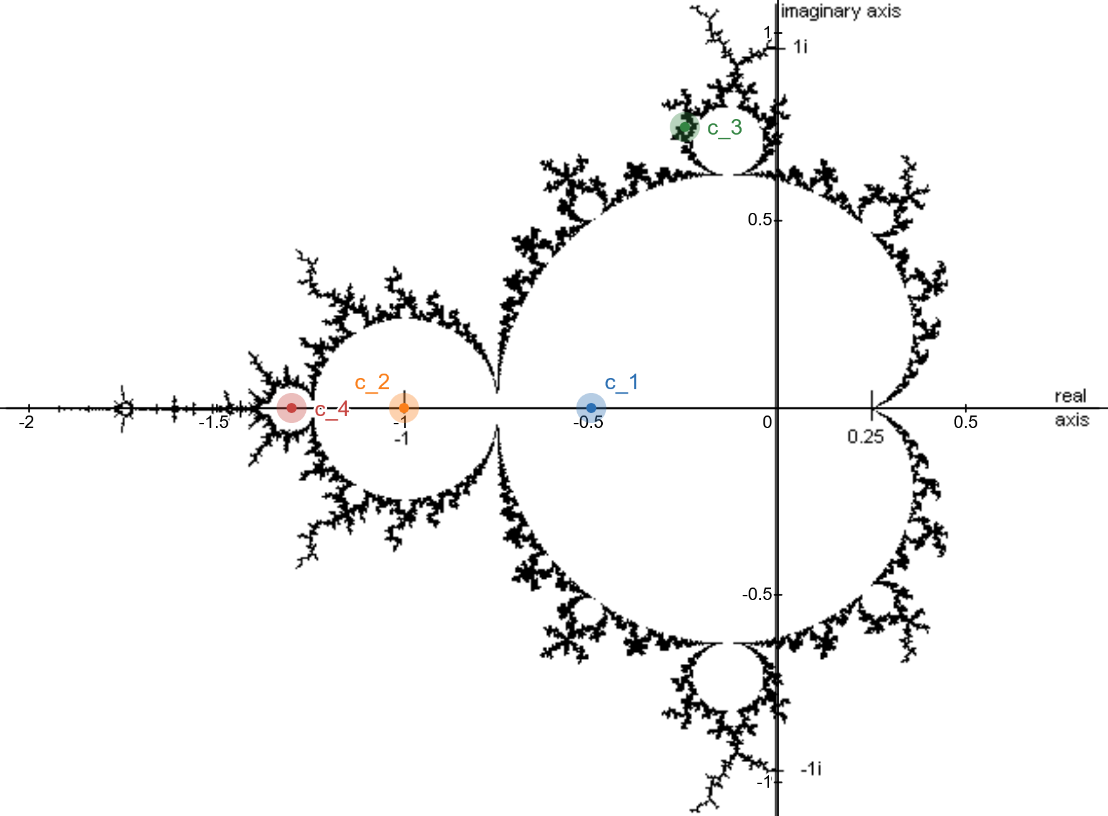
\includegraphics[width=\textwidth]{papers/julia/imgs/mandelbrot_punkte.png}

    \caption{Beispielspunkte in verschiedenen Regionen der Mandelbrot-Menge}
    \label{julia:beispiele_aussehen_mandel}
\end{figure}


\subsection{Verallgemeinerungen}
Die Mandelbrot-Menge lässt sich auf verschiedene Arten verallgemeinern.
In diesem Abschnitt werden einige davon beschrieben.

\subsubsection{Multibrot-Mengen}
Multibrot-Mengen entstehen, wenn man statt einer quadratischen Funktion Polynome eines beliebigen Grades betrachtet
\index{Multibrot-Mengen}%
\begin{equation*}
    f_c(z) = z^d + c.
\end{equation*}
Beispiele davon sind in Abbildung \ref{julia:fig:multibrot_mengen} dargestellt.
Dies kann weiter verallgemeinert werden, indem negative und rationale Zahlen als Exponent $d$ erlaubt werden.
\begin{figure}
    \centering
    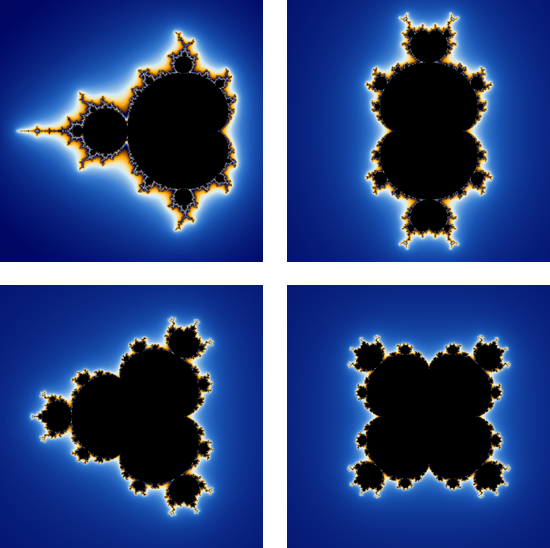
\includegraphics[width=\textwidth]{papers/julia/imgs/multibrot.png}

    \caption{Multibrot-Mengen für Polynome der Grade $2$, $3$, $4$ und $5$}
    \label{julia:fig:multibrot_mengen}
\end{figure}

\subsubsection{Höhere Dimensionen}
Statt den komplexen Zahlen kann auch mit \emph{Quaternionen} gearbeitet werden, diese sind die vierdimensionale Erweiterung der komplexen Zahlen.
\index{Quaternionen}%
Ein Quaternion wird als $q = a + bi + cj + dk$ notiert, mit $i^2 = j^2 = k^2 = ijk = -1$ und $i \ne j \ne k$.

Die vierdimensionale Mandelbrot-Menge kann dann in eine dreidimensionale Struktur projiziert werden, was jedoch relativ uninteressant ist, da es sich lediglich um die Mandelbrot-Menge, rotiert um die reelle Achse handelt \cite{julia:quaternionen}.

\subsubsection{Nicht-analytische Funktionen}
Statt holomorphen Funktionen können auch nicht-holomorphe bzw. nicht-analytische Funktionen verwendet werden.

Ein bekanntes Beispiel ist das Tricorn-Fraktal, dabei wird die Rekursion
\index{Tricorn-Fraktal}%
\begin{equation*}
    z_{n+1} = \overline{z_n}^2 + c
\end{equation*}
verwendet.
Bevor $z_n$ quadriert wird, wird die komplexe Konjugation berechnet.

Ein weiteres Beispiel ist das Burning-Ship-Fraktal, welches durch die Rekursion
\index{Burning-Ship-Fraktal}%
\begin{equation*}
    z_{n+1} = \left(|\text{Re}(z_n)| + i\,|\text{Im}(z_n)|\right)^2 + c
\end{equation*}
entsteht.
Anders als bei der Mandelbrot-Menge werden hier die Beträge des Real- und Imaginärteils berechnet, bevor quadriert wird.
